\todo[color=red]{Das große Problem ist: Wir haben das $U_0$ nicht bestimmt. Ich habe es einfach auf 20 Volt geschätzt. Es scheint jedoch etwas kleiner gewesen zu sein.}

\subsection{Berechnung der Zeitkonstanten}
\subsubsection{... durch die Aufladekurve des Kondensators}
Um die Gleichung für die lineare Regression zu erhalten, wird Formel \eqref{eq:aufladen} umgeformt zu
\begin{equation}
\ln(U_C - U_0) = -\frac{1}{RC} t + \ln(U_0) \quad .
\end{equation}
Die angelegte Spannung $U_0$ entspricht der Peak to Peak Amplitude der Rechteckspannung.
\begin{align*}
	U_0 = \SI{19.4}{\volt}
\end{align*}
In Abbildung \ref{fig:spannung1} ist die Differenz der angelegten Spannung und der Kondensatorspannung $U_0 - U_C$ halblogarithmisch über die Zeit aufgetragen. Eine lineare Ausgleichsrechnung der Form
\begin{equation}
\ln(U_C - U_0) = m \cdot t + b
\end{equation} an die in Tabelle \ref{tab:aufladekurve} dargestellten Werte mittels Python liefert:
\begin{align}
	&m = \SI{-1290.4(150)}{\second} \\
	&b = \num{3.011(25)} \\
	&\text{Zeitkonstante:} \quad RC = - \frac{1}{m} = \SI{0.775(9)e-3}{\second} \\
	&\text{Berechnete Ausgangsspannung:} \quad U_{\text{reg}} = e ^b \, \si{\volt} = \SI{20,3(5)}{\volt} \label{eq:u_reg}
\end{align}

\begin{figure}[h!]
	\centering
	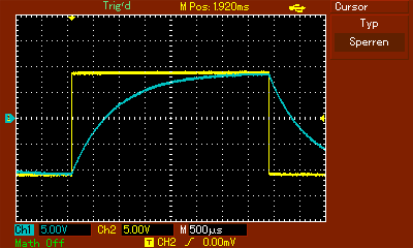
\includegraphics[width=0.6\textwidth]{aufladekurve.png}
	\caption{Aufladekurve des Kondensators bei angelegter Rechteckspannung}
	\label{fig:aufladekurve}
\end{figure} 
\begin{figure}[h!]
	\centering
	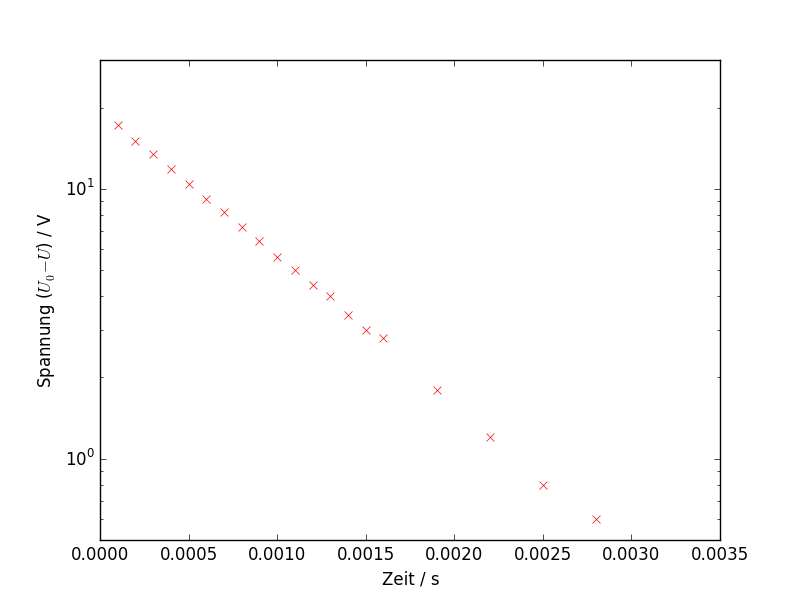
\includegraphics[width=0.7\textwidth]{Spannung1.png}
	\caption{Spannungsdifferenzen mit Messunsicherheit halblogarithmisch aufgetragen}
	\label{fig:spannung1}
\end{figure} 

\begin{figure}[h!]
	\centering
	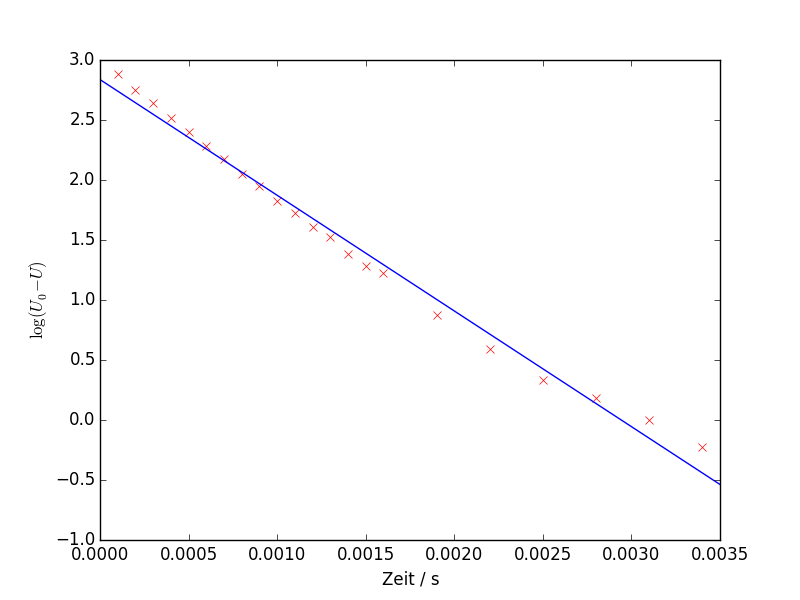
\includegraphics[width=0.7\textwidth]{Spannung2.png}
	\caption{Ausgleichsgerade zur Bestimmung der Zeitkonstanten mit Messunsicherheiten}
	\label{fig:Spannung2}
\end{figure} 
\begin{figure}[h!]
	\centering
	\captionof{table}{Werte der Aufladekurve}
	\begin{tabular}{c|c|c}
		Zeit in \si{\milli\second}& $\ln(U_0-U)$ & Fehler in $10^{-2}\ln(\si{\volt})$ \\
		\hline
		0.1 &  2.84 &  0.12 \\
		0.2 &  2.71 &  0.13 \\
		0.3 &  2.6  &  0.15 \\
		0.4 &  2.47 &  0.17 \\
		0.5 &  2.34 &  0.19 \\
		0.6 &  2.22 &  0.22 \\
		0.7 &  2.1  &  0.24 \\
		0.8 &  1.97 &  0.28 \\
		0.9 &  1.86 &  0.31 \\
		1.0 &  1.72 &  0.36 \\
		1.1 &  1.61 &  0.40  \\
		1.2 &  1.48 &  0.45 \\
		1.3 &  1.39 &  0.50  \\
		1.4 &  1.22 &  0.59 \\
		1.5 &  1.1  &  0.67 \\
		1.6 &  1.03 &  0.71 \\
		1.9 &  0.59 &  1.11 \\
		2.2 &  0.18 &  1.67 \\
		2.5 & -0.22 &  2.50  \\
		2.8 & -0.51 &  3.33 \\
		3.1 & -0.92 &  5.00   \\
		3.4 & -1.61 & 10.00    \\
	\end{tabular}
	\label{tab:aufladekurve}
	\\
	\vspace{1cm}
	\begin{tabular}{ll}
		Messunsicherheit der Zeit: & \SI{3e-5}{\second}
	\end{tabular}
\end{figure}



\clearpage
\subsubsection{... durch die frequenzabhängige Amplitude bei periodischer Anregung}
\begin{figure}[h!]
\centering
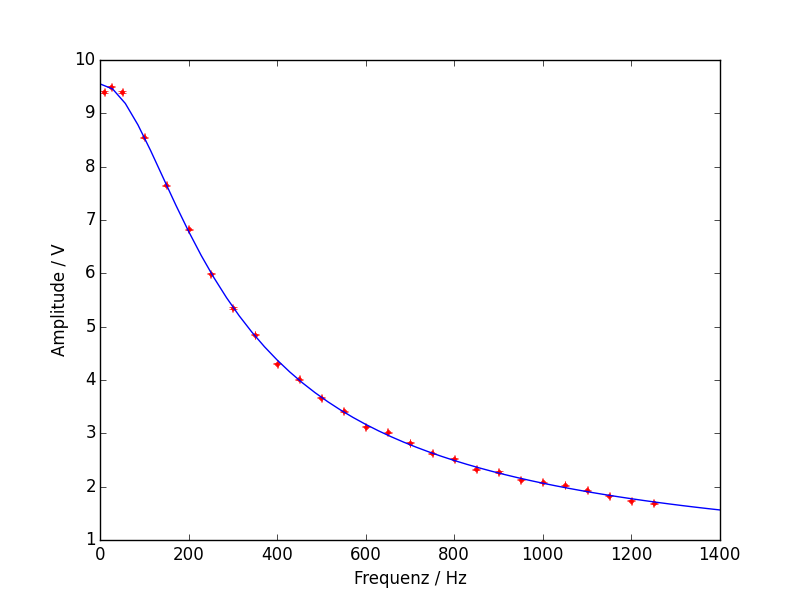
\includegraphics[width=0.7\textwidth]{Amplitude.png}
\caption{Amplitude in Abhängigkeit der Frequenz mit Messunsicherheiten}
\label{fig:amplitude}
\end{figure} 

Noch Formel \eqref{eq:amplitude} ist ersichtlich, dass die Amplitude ungefähr mit $\frac{1}{\nu}$ abfällt. Hier wird mittels Python ein nichtlinearer Fit durchgeführt:
\begin{equation}
A(\nu) = \frac{b}{\sqrt{1+(2\pi \nu)^2 e)}} + d
\end{equation}
Wobei $b$ der Amplitude der angelegten Sinusfunktion sein sollte, $e$ die Wurzel der Zeitkonstante und d einen Offstets des Gerätes angeben würde, falls es einen gibt.
Die Werte aus Tabelle \ref{tab:amplitude} liefern folgende Fit-Parameter:
\begin{align}
	b &=  \SI{9,28(4)}{\volt} \label{eq:b} \\
	c &=  \SI{6.51(14)e-7}{\second\squared} \\
	d &=  \SI{0.27(3)}{\volt} \label{eq:d}\\
	RC &= \SI{0,807(9)e-3}{\second}
\end{align}

\begin{figure}[h!]
	\centering
	\captionof{table}{Amplitude in Abhängigkeit von der Frequenz}
	\begin{tabular}{c|c}
		Frequenz in \si{\hertz}& Amplitude in \si{\volt} \\
		\hline
	10 & 9.40  \\
	25 & 9.50  \\
	50 & 9.40  \\
	100 & 8.55 \\
	150 & 7.65 \\
	200 & 6.83 \\
	250 & 5.99 \\
	300 & 5.35 \\
	350 & 4.85 \\
	400 & 4.30  \\
	450 & 4.01 \\
	500 & 3.66 \\
	550 & 3.42 \\
	600 & 3.12 \\
	650 & 3.02 \\
	700 & 2.82 \\
	750 & 2.62 \\
	800 & 2.52 \\
	850 & 2.33 \\
	900 & 2.28 \\
	950 & 2.13 \\
	1000 & 2.08 \\
	1050 & 2.03 \\
	1100 & 1.93 \\
	1150 & 1.83 \\
	1200 & 1.74 \\
	1250 & 1.68 \\
	\end{tabular}
	\label{tab:amplitude}
	\\
	\vspace{1cm}
	\begin{tabular}{ll}
		Messunsicherheit der Frequenz & \SI{1}{\hertz} \\
		Messunsicherheit der Amplitude & \SI{0.01}{\volt}
	\end{tabular}	
\end{figure}



\clearpage
\subsubsection{... durch die frequenzabhängige Phasenverschiebung}
Auch in diesem Abschnitt wird durch eine nichtlineare Regression die Zeitkonstante Bestimmt. Die Phasendifferenz zwischen Eingangs- und Ausgangssignal bei einer Sinusspannung sind nach Formel \eqref{eq:phase} Frequenzabhängig. Die Phasendifferenz wird mit Oszilloskop ermittelt, indem der Abstand $a$ zweier Kurven bei bekannter Frequenz $\nu$ gemessen wird
\begin{equation}
\phi = 2 \pi a \nu \quad .
\end{equation}
Die Regression an den Acrustangens (Abb. \ref{fig:phasenverschub}) mit dem Parameter $b$ erfolgt nach
\begin{equation}
\phi (\nu) = \arctan(-2\pi \nu b) \quad .
\end{equation}
Und liefert mit den Werten aus Tabelle \ref{tab:phasenverschub} die Zeitkonstante
\begin{equation}
RC = b = \SI{-0.782(14)e-3}{\second} \quad.
\end{equation}
Wobei das negative Vorzeichen aus der Definition der Winkel entsteht und somit ignoriert werden kann.

\begin{figure}[h!]
	\centering
	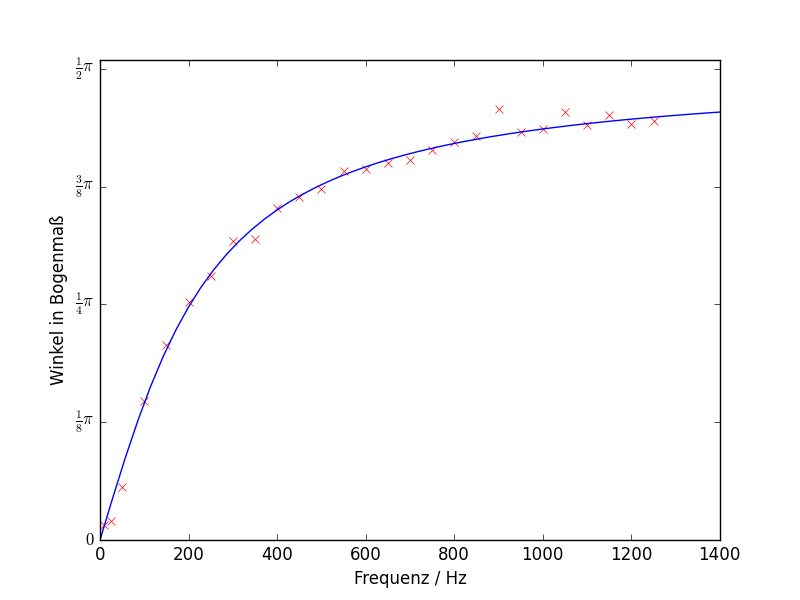
\includegraphics[width=0.7\textwidth]{Phasenverschub1.png}
	\caption{Amplitude in Abhängigkeit der Frequenz mit Messunsicherheiten}
	\label{fig:phasenverschub}
\end{figure} 


\begin{figure}[h!]
	\centering
	\captionof{table}{Frequenz und Phasendifferenz}
	\begin{tabular}{c|c|c|c}
	Frequenz in \si{\hertz}&  $a$ \si{\milli\second} & Winkel in Bogenmaß & Fehler in $10^{-2}\si{\radian}$ \\
		\hline
		10 & 0.80  & 0.05 & 0.51 \\
		25 & 0.40  & 0.06 & 0.28 \\
		50 & 0.56 & 0.18 & 0.43 \\
		100 & 0.74 & 0.46 & 0.68 \\
		150 & 0.69 & 0.65 & 0.87 \\
		200 & 0.63 & 0.79 & 1.08 \\
		250 & 0.56 & 0.88 & 1.3  \\
		300 & 0.53 & 1.00    & 1.54 \\
		350 & 0.46 & 1.00    & 1.78 \\
		400 & 0.44 & 1.11 & 2.03 \\
		450 & 0.40 & 1.14 & 2.28 \\
		500 & 0.37 & 1.17 & 2.52 \\
		550 & 0.36 & 1.23 & 2.77 \\
		600 & 0.33 & 1.24 & 3.02 \\
		650 & 0.31 & 1.26 & 3.27 \\
		700 & 0.29 & 1.27 & 3.52 \\
		750 & 0.28 & 1.30  & 3.77 \\
		800 & 0.26 & 1.33 & 4.02 \\
		850 & 0.25 & 1.35 & 4.28 \\
		900 & 0.25 & 1.44 & 4.53 \\
		950 & 0.23 & 1.36 & 4.78 \\
		1000 & 0.22 & 1.37 & 5.03 \\
		1050 & 0.22 & 1.43 & 5.28 \\
		1100 & 0.20  & 1.38 & 5.53 \\
		1150 & 0.20  & 1.42 & 5.78 \\
		1200 & 0.18 & 1.39 & 6.03 \\
		1250 & 0.18 & 1.40  & 6.28 \\
		\end{tabular}
	\label{tab:phasenverschub}
	\\
	\vspace{1cm}
	\begin{tabular}{ll}
		Messunsicherheit Frequenz & \SI{1}{\hertz} \\
		Messunsicherheit Zeitdifferenz $a$ & \SI{8e-6}{\second}
	\end{tabular}	
\end{figure}

\clearpage
\subsection{Polarplot der Amplitude über die Phasendifferenz}
Unter Berücksichtigung der Beziehung $\tan^2(\phi) = \omega ^2 R^2 C^2$ kann die Amplitude in Abhängigkeit von der Phasendifferenz $\phi$ ausgedrückt werden
\begin{equation}
A(\phi) = \frac{U_0}{\sqrt{(1+\tan^2(\phi))}} = U_0 \cos(\phi)
\end{equation}
In Abbildung \ref{fig:phasenverschub2} ist die theoretische Kurve in einem Polarkoordinatensystem und zusätzlich jeder zweite gemessene Wert der Phasendifferenz (siehe Tabelle \ref{tab:phasenverschub}) gezeigt.

\begin{figure}[h!]
	\centering
	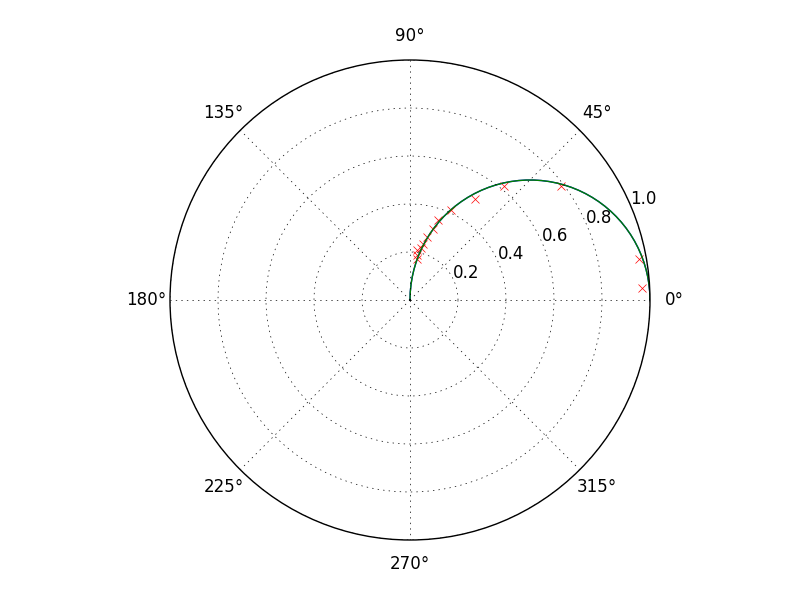
\includegraphics[width=0.7\textwidth]{Phasenverschub2.png}
	\caption{Amplitude über die Phasendifferenz}
	\label{fig:phasenverschub2}
\end{figure} 



\clearpage
\subsection{RC-Glied als Integrator}
In diesem Abschnitt wird die Verwendung eines RC-Gliedes als Integrator überprüft. Integriert wird eine Rechteck, eine Cosinus- und eine Dreieckspannung. Das jeweilige Eingangs- und Ausgangssignal (Integral zum Eingangssignal) ist in den Abbildungen \ref{fig:integral1}, \ref{fig:integral2} und \ref{fig:integral3} zu sehen.
\begin{align}
	&\text{Rechteckspannung:} \quad f_R(t) = \begin{cases}
		c, & 0\leq t < a \\
		-c, & -a < t < 0
	\end{cases} \\
&\text{Cosinusspannung:} \quad f_C(t) = \cos{t} \\
	&\text{Dreieckspannung:} \quad f_D(t) = \begin{cases}
		\frac{2c}{a} t-c, & 0\leq t < a \\
	-\frac{2c}{a} t-c, & -a < t < 0
	\end{cases} \\
\end{align}

Die zugehörigen Stammfunktionen sind:
\begin{align}
	&F_R(t) = \begin{cases}
		\frac{2c}{a} t - c, & 0\leq t < a \\
		-\frac{2c}{a} t - c, & -a < t < 0
	\end{cases} \\
	&F_C(t) = -\sin{t} \\
	&F_D(t) = \begin{cases}
		\frac{c}{a} t^2-ct + c_2, & 0\leq t < a \\
		-\frac{c}{a} t^2-ct - c_2, & -a < t < 0
	\end{cases} \\
\end{align}


\begin{figure}[h!]
	\centering
	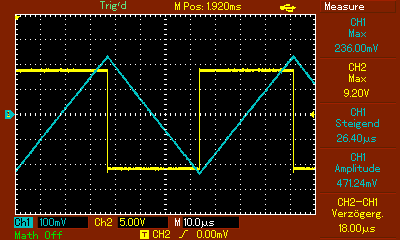
\includegraphics[width=0.6\textwidth]{MAP002.png}
	\caption{Integration einer Rechteckspannung}
	\label{fig:integral1}
\end{figure} 

\begin{figure}[h!]
	\centering
	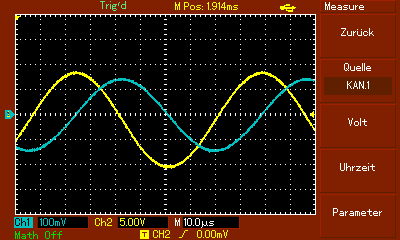
\includegraphics[width=0.6\textwidth]{MAP003.png}
	\caption{Integration einer negativen Cosinusspannung}
	\label{fig:integral2}
\end{figure} 

\begin{figure}[h!]
	\centering
	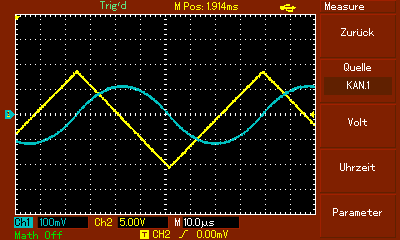
\includegraphics[width=0.6\textwidth]{MAP004.png}
	\caption{Integration einer Dreieckspannung}
	\label{fig:integral3}
\end{figure} 






	
